\documentclass[12pt]{article}

\usepackage[onehalfspacing]{setspace}
\usepackage{rotating}
\usepackage{caption}
\usepackage{lscape}
\usepackage{epstopdf}
\usepackage{graphicx}
\usepackage{amsmath}
\usepackage{threeparttable}
\usepackage[utf8]{inputenc}
\usepackage{lmodern,textcomp}
\usepackage{floatrow}
\usepackage{tabularx}
\usepackage{float}
\usepackage{longtable}

\usepackage{natbib}
\bibliographystyle{apalike}

\usepackage{eurosym}
\usepackage{amssymb}
\usepackage{amsmath}
\usepackage{graphics}

\usepackage{verbatim}
\usepackage{multirow}
\usepackage{floatrow}

	\floatsetup[table]{capposition=top}

\usepackage{longtable}
\usepackage{pdflscape}

\usepackage[paperwidth=210mm,paperheight=297mm,left=27mm,right=27mm,top=25mm,bottom=25mm]{geometry}

\usepackage[dvipsnames]{xcolor}
\usepackage{color, colortbl}

	\definecolor{Gray}{gray}{0.9}
	\definecolor{LightCyan}{rgb}{0.88,1,1}

\usepackage{afterpage}

\usepackage{soul}

\usepackage[hyphens]{url}
\usepackage[colorlinks,breaklinks=true]{hyperref}

\hypersetup{pdfnewwindow=true}

\hypersetup{
     colorlinks   = true,
     citecolor    = black
}

\hypersetup{linkcolor=blue!75!black}
\hypersetup{urlcolor=blue!75!black}
\hypersetup{filecolor=blue!75!black}
\hypersetup{citecolor=black}

\begin{document}

\title{Lorem ipsum dolor sit amet, consectetur adipiscing elit\thanks{Eu nisl nunc mi ipsum faucibus vitae aliquet nec. Diam volutpat commodo sed egestas egestas fringilla. Id diam maecenas ultricies mi eget mauris. Ullamcorper malesuada proin libero nunc consequat.}}
\author{Z. Petra\thanks{%
UNS.}\quad P. Todd\thanks{UUSTT.}}

\maketitle


\begin{abstract}
\singlespacing {\small 
Lorem ipsum dolor sit amet, consectetur adipiscing elit, sed do eiusmod tempor incididunt ut labore et dolore magna aliqua. Ac turpis egestas integer eget. Faucibus vitae aliquet nec ullamcorper sit amet risus nullam. Sit amet risus nullam eget felis eget nunc lobortis. Et netus et malesuada fames ac turpis egestas maecenas. Sed faucibus turpis in eu mi bibendum neque. Arcu odio ut sem nulla pharetra diam. Faucibus ornare suspendisse sed nisi lacus sed viverra. Sodales ut etiam sit amet nisl purus in mollis. Enim nec dui nunc mattis enim ut tellus. Id faucibus nisl tincidunt eget nullam non. Donec enim diam vulputate ut pharetra sit.}
\end{abstract}

\textbf{Keywords:} Nunc mattis enim ut tellus elementum sagittis.

\textbf{JEL Classification:} \textit{J38, L25}

\newpage

\section{Introduction} \label{sec:introduction}

Lorem ipsum dolor sit amet, consectetur adipiscing elit, sed do eiusmod tempor incididunt ut labore et dolore magna aliqua. Odio tempor orci dapibus ultrices in iaculis nunc. Ultrices dui sapien eget mi proin. Justo laoreet sit amet cursus sit. Euismod in pellentesque massa placerat duis. Amet nulla facilisi morbi tempus iaculis urna id volutpat lacus. At elementum eu facilisis sed odio morbi quis. Consequat ac felis donec et odio pellentesque diam volutpat. Enim neque volutpat ac tincidunt vitae semper quis lectus nulla. Quisque non tellus orci ac auctor augue mauris augue neque. Nullam non nisi est sit amet facilisis magna etiam. Etiam dignissim diam quis enim lobortis scelerisque fermentum dui. Gravida arcu ac tortor dignissim convallis aenean.

Commodo elit at imperdiet dui accumsan. Amet venenatis urna cursus eget. Magnis dis parturient montes nascetur ridiculus mus mauris vitae ultricies. Sagittis nisl rhoncus mattis rhoncus urna. Vitae et leo duis ut diam quam nulla. At tempor commodo ullamcorper a lacus vestibulum. Gravida cum sociis natoque penatibus et magnis dis parturient montes. Nunc sed augue lacus viverra vitae congue eu. Interdum posuere lorem ipsum dolor sit amet consectetur adipiscing. Ultrices sagittis orci a scelerisque purus semper eget duis at. Ullamcorper eget nulla facilisi etiam dignissim diam. Pulvinar neque laoreet suspendisse interdum consectetur libero id. Nulla facilisi morbi tempus iaculis urna. Massa tincidunt dui ut ornare lectus sit amet est placerat.

Quis varius quam quisque id \cite{draca2011minimum}. Nisi porta lorem mollis aliquam. Tellus mauris a diam maecenas. Porta non pulvinar neque laoreet suspendisse interdum. Urna neque viverra justo nec ultrices dui. Mauris ultrices eros in cursus turpis massa tincidunt dui ut. Id aliquet lectus proin nibh nisl condimentum id venenatis. Hendrerit dolor magna eget est lorem ipsum dolor. Praesent tristique magna sit amet. Nullam non nisi est sit. Suspendisse sed nisi lacus sed viverra tellus in hac. \cite{harasztosi2019pays} for a large increase in the Hungarian minimum wage in 1997-2004 Dignissim enim sit amet venenatis urna cursus eget. Duis at consectetur lorem donec massa sapien faucibus et. Lectus mauris ultrices eros in cursus turpis. Donec enim diam vulputate ut. Accumsan in nisl nisi scelerisque eu ultrices vitae auctor eu. Vitae elementum curabitur vitae nunc sed velit dignissim sodales. Ipsum dolor sit amet consectetur adipiscing elit ut aliquam purus. Elit at imperdiet dui accumsan sit amet. Nunc congue nisi vitae suscipit.




\begin{figure}[ht]
\begin{minipage}{.75\linewidth}
\caption{Share of financially distressed firms}\label{fig:FDF}
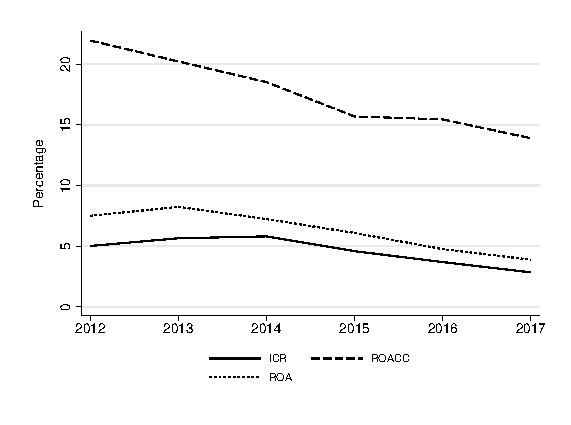
\includegraphics[width=\linewidth]{figures/share_zombies.eps}
\footnotesize
\emph{Source:} Authors' computations using data from SCIE.
\end{minipage}{}
\end{figure}

The fragile condition of financially distressed firms raised concerns about the effects of minimum wage policies. Minimum wage increases may induce a further deterioration of the financial condition of those firms, which may lead them to reduce employment and even to close down. 
Business leaders publicly expressed their concerns on the effects of wage cost increases, namely in sectors where there is a high minimum wage incidence and labor costs weigh heavily in total costs. 

The minimum wage in Portugal is set for a month of work and the full time weekly hours, with a maximum legal working week of 40 hours, are defined in the collective bargaining agreement. Between 2014 and 2017, the minimum wage increased 14.8\%. In October 2014, minimum wage increased from 485 to 505 euros, a 4\% change. Notwithstanding being a small increase, the percentage of workers receiving minimum wage jumped from 13.2\% to 19.6\%.\footnote{The numbers mentioned in this part of the text come from a report on the minimum wage in Portugal published by the Portuguese Ministry of Labor.} 


\begin{equation}\label{eq:prci}
PRCI_{i t} = \frac{Potencial\; wage\; bill_{i,t+1}\; -\; Current\; wage\; bill_{it}}{Total\; costs_{it}} \times 100
\end{equation}

This equation tells that the 'potential relative cost increase' associated with a minimum wage rise is the relative change in total costs that the firm would face in year $t$ if the firm had to pay in year $t$ the year $t+1$ minimum wage, while maintaining the same productive structure, namely, not adjusting the composition, nor the size, of its labor force in view of the minimum wage increase.  
By computing the 'potential relative cost increase' we take into consideration the fact that the importance of labor costs varies across industries and firms.


\section{Empirical analysis} \label{sec:empirical}




\subsection{Econometric strategy}



To evaluate the impact of minimum wage increases on firm exit, we begin by estimating a logit model that accounts for firms' unobserved heterogeneity and in which the dependent variable is the probability that firm $i$ will close down in period $t+1$: 

\begin{equation}\label{eq:dead-prob}
 P(E_{i, t+1}=1|\theta_{i t}) = \lambda(\theta_{i t}) = \frac{\exp{(\theta_{i 
t})}}{1+\exp{(\theta_{i t})}} 
\end{equation}
\begin{equation}\label{eq:dead-formula}
 \theta_{i t} = \beta_1 PRCI_{i t} + \beta_2 FDF_{i,t-1} + \beta_3 PRCI_{i t} FDF_{i,t-1} + 
\beta_4^\prime X_{i t} + \eta_i 
\end{equation}

In equation (\ref{eq:dead-prob}), $E_{i, t+1}$ is a dummy variable that equals 1 if firm $i$ exited during year $t+1$ and equals 0 otherwise. 



%------------------------


\subsection{Results}

Lorem ipsum dolor sit amet, consectetur adipiscing elit, sed do eiusmod tempor incididunt ut labore et dolore magna aliqua. At tempor commodo ullamcorper a lacus vestibulum sed. Eu consequat ac felis donec et odio pellentesque diam. Eget nunc scelerisque viverra mauris in. Hendrerit gravida rutrum quisque non tellus orci ac auctor. Egestas dui id ornare arcu odio ut sem nulla. Mauris commodo quis imperdiet massa. Tempor id eu nisl nunc mi ipsum faucibus. Nibh sed pulvinar proin gravida hendrerit. Et egestas quis ipsum suspendisse ultrices gravida dictum fusce ut. Arcu dictum varius duis at consectetur. Nec dui nunc mattis enim ut tellus elementum sagittis. Amet justo donec enim diam vulputate ut. Nulla aliquet enim tortor at. Ac turpis egestas maecenas pharetra convallis posuere morbi.

Pharetra et ultrices neque ornare aenean euismod elementum nisi. Senectus et netus et malesuada. Felis eget nunc lobortis mattis aliquam faucibus. Quis commodo odio aenean sed. Facilisis gravida neque convallis a cras semper. Augue mauris augue neque gravida in fermentum. Eget duis at tellus at urna condimentum mattis pellentesque. Odio morbi quis commodo odio aenean sed adipiscing diam. Odio tempor orci dapibus ultrices in iaculis nunc sed. Augue mauris augue neque gravida in fermentum et. Sed odio morbi quis commodo odio aenean sed. Elit pellentesque habitant morbi tristique. Arcu bibendum at varius vel pharetra vel. Justo eget magna fermentum iaculis eu non diam. Quis auctor elit sed vulputate. Mattis rhoncus urna neque viverra. Nullam non nisi est sit amet facilisis magna etiam. Amet consectetur adipiscing elit ut aliquam purus sit amet. Pulvinar etiam non quam lacus suspendisse faucibus.

\afterpage{%
    \clearpage% Flush earlier floats (otherwise order might not be correct)
%    \thispagestyle{empty}% empty page style (?)
    \begin{landscape}% Landscape page
    \topskip0pt
    \vspace*{\fill}
    \begin{table}[H]
\centering
\caption{Profitability, employment and exit}\label{tb:results}
   \begin{center}
\resizebox{1.0\textwidth}{!}
   {{
\def\sym#1{\ifmmode^{#1}\else\(^{#1}\)\fi}
\begin{tabular}{l*{10}{c}}
\hline
            &\multicolumn{2}{c}{Profit}&\multicolumn{2}{c}{Employment}&\multicolumn{2}{c}{Exit (Logit)}&\multicolumn{2}{c}{Exit (LPM - A)}&\multicolumn{2}{c}{Exit (LPM - B)}\\\hline
    &     (1) &     (2)    &     (3)&     (4)&      (5)&      (6)&      (7)&      (8)&      (9)&      (10)\\\hline
& \multicolumn{10}{c}{Panel A: Baseline} \\ \hline
PRCI        &     -9.8842\sym{***}&     -9.9816\sym{***}&     -3.9870\sym{***}&     -5.5859\sym{***}&      4.4586\sym{***}&      4.3970\sym{***}&      0.0979         &      0.1014         &      0.0388\sym{***}&      0.0388\sym{***}\\
            &     (3.197)         &     (3.179)         &     (1.458)         &     (2.000)         &     (0.280)         &     (0.255)         &     (0.074)         &     (0.075)         &     (0.013)         &     (0.012)         \\
\hline\hline
& \multicolumn{10}{c}{Panel B: Full specification}\\\hline
PRCI        &     -9.4955\sym{***}&     -9.5863\sym{***}&     -3.7775\sym{***}&     -5.3323\sym{***}&      4.4094\sym{***}&      4.3452\sym{***}&      0.5644\sym{***}&      0.5610\sym{***}&      0.0370\sym{***}&      0.0370\sym{***}\\
            &     (3.144)         &     (3.128)         &     (1.428)         &     (1.969)         &     (0.220)         &     (0.248)         &     (0.051)         &     (0.050)         &     (0.012)         &     (0.012)         \\
[1em]
Lag FDF       &     -3.7604\sym{***}&     -3.7798\sym{***}&     -1.3050\sym{**} &     -0.9133         &      0.5279\sym{***}&      0.5425\sym{***}&      0.1467\sym{***}&      0.1490\sym{***}&      0.0149\sym{***}&      0.0151\sym{***}\\
            &     (0.895)         &     (0.899)         &     (0.641)         &     (0.670)         &     (0.091)         &     (0.073)         &     (0.023)         &     (0.023)         &     (0.004)         &     (0.004)         \\
[1em]
PRCI $ \times $ Lag FDF&    -11.0203\sym{***}&    -11.1090\sym{***}&     -6.0761\sym{***}&     -7.4045\sym{***}&      0.3881         &      0.4083         &      0.1516\sym{**} &      0.1533\sym{**} &      0.0503\sym{***}&      0.0507\sym{***}\\
            &     (2.871)         &     (2.905)         &     (1.592)         &     (1.886)         &     (0.341)         &     (0.317)         &     (0.061)         &     (0.061)         &     (0.012)         &     (0.012)         \\\hline
\multicolumn{11}{p{25.0cm}}{\footnotesize Notes: Standard errors are clustered at the firm level for models (1)-(4) and (7)-(10); for models (5) and (6) standard errors are computed by bootstrap. Significance levels: *, 10\%; **, 5\%; ***, 1\%. The dependent variables are identified in each set of columns. Panel A reports estimates for a baseline model without the financial distress indicator and its interaction with PRCI; in Panel B those variables are included.
LPM stands for Linear Probability Model. The estimations reported in columns (1), (3), (5) and (7) include additionally the following control variables: part-time workers, fixed-term workers, overtime labor, relative labor costs, exports weight, leverage ratio,valued-added per hour, short-term debt, long-term debt and the number of workers and its square. Results under Exit (Logit) are estimated by conditional logit while the remaining models account for firm unobserved heterogeneity using the fixed effects estimator. The number of observations is 27998 for columns (5), (6), (7) and (8). The number of observations is 368085 for the remaining estimations. The model Exit (LPM - A) is estimated with the same sample as the model Exit (Logit) model. The model Exit (LPM-B) is estimated with the same sample as the Profit and Employment models.}\\
\end{tabular}
}
}
   \end{center}
\end{table}
    \vspace*{\fill}


    \end{landscape}
}


As an alternative to the logit functional form, in columns (7) and (8) of Table \ref{tb:results} we report the estimates obtained using the linear probability model, estimated in the same sample as the logit model, i.e., the sample of firms that did exit during 2014-2017. 
As in the logit model, the coefficients are positive and statistically significant at the 1\% significance level. 
Hence, qualitatively the results are the same as in the logit model. 
Quantitatively, the change in the probability of exit assigned to the minimum wage rise is a bit lower than in the logit model --- see the mid-section of Table \ref{tb:impact}. 
This is especially so for non-financially distressed firms, for which this model estimates impacts that are not much higher than half of the logit estimates. 
Nevertheless, the magnitude of the average impact is still reasonably large, reaching 16 percentage points in 2016. 
For financially distressed firms, the linear model also produces lower estimates of the average impact than the logit model, but the difference is relatively small (less than six percentage points). 
In short, the linear probability model attenuates the magnitude of the average impact of the minimum wage increases, but is in line with the conclusions derived from the logit model. 


\begin{table}[ht]
\caption{Impact on the probability of exit (\%) of the average firm}\label{tb:impact}
    \begin{center}
%\resizebox{0.5\textwidth}{!}
    {\begin{tabular}{lcccc}
\hline & 2013 & 2014 & 2015 & 2016 \\ \hline \\
Logit &  &  &  &  \\ 
\hspace*{0.2cm}Non-FDF & 5.0 & 13.4 & 24.5 & 27.5 \\ 
\hspace*{0.2cm}FDF & 5.6 & 15.9 & 27.3 & 30.4 \\ 
 &  &  &  &  \\ 
LPM – A (firms that exited) &  &  &  &  \\ 
\hspace*{0.2cm}Non-FDF & 2.6 & 7.2 & 14.0 & 16.2 \\ 
\hspace*{0.2cm}FDF & 3.7 & 11.1 & 21.9 & 25.9 \\ 
 &  &  &  &  \\ 
LPM – B (all firms) &  &  &  &  \\ 
\hspace*{0.2cm}Non-FDF & 0.2 & 0.5 & 1.0 & 1.2 \\ 
\hspace*{0.2cm}FDF & 0.6 & 1.7 & 3.4 & 4.1 \\ 
\hline
\multicolumn{5}{p{0.65\textwidth}}{\footnotesize Notes: The numbers are the difference in the probability of exit between a firm with a value for the treatment variable equal to the average of that variable for the same category of firms (non-FDF or FDF) in each year, and a firm with the same characteristics but a zero value for the treatment variable. ``Logit'' uses the estimates in column (5) of Table \ref{tb:results}. ``LPM - A'' and ``LPM - B'' use the estimates in columns (7) and (9), respectively.} 
\end{tabular}
}
    \end{center}
\end{table}



We also estimated the linear probability model on the full sample of firms. 
The results are in columns (9) and (10) of Table \ref{tb:results}. 
Extending the sample to include the firms that did not exit during 2014-2017 makes some difference. 
First, the dummy for financially distressed firms is no longer statistically significant. 
Second, and more importantly, the attenuation effect detected above is now much stronger. 
The estimated average impact is now in the range $0.2-1.2$ for non-financially distressed firms, and in the range $0.6-4.1$ for financially distressed firms.




\section{Conclusion} \label{sec:conclusion}

Lorem ipsum dolor sit amet, consectetur adipiscing elit, sed do eiusmod tempor incididunt ut labore et dolore magna aliqua. Eget magna fermentum iaculis eu non diam. Nibh cras pulvinar mattis nunc sed. Purus in mollis nunc sed id. Molestie nunc non blandit massa enim nec. Est ante in nibh mauris cursus mattis molestie. Pulvinar mattis nunc sed blandit libero volutpat sed cras ornare. Vulputate enim nulla aliquet porttitor lacus luctus accumsan tortor posuere. Facilisis volutpat est velit egestas dui id ornare arcu. Hac habitasse platea dictumst vestibulum rhoncus. Sollicitudin nibh sit amet commodo nulla facilisi. Purus ut faucibus pulvinar elementum integer enim. Penatibus et magnis dis parturient montes. Cursus eget nunc scelerisque viverra mauris. Blandit turpis cursus in hac.

Commodo nulla facilisi nullam vehicula ipsum a arcu. Pulvinar etiam non quam lacus suspendisse faucibus. Feugiat pretium nibh ipsum consequat nisl vel pretium. Luctus venenatis lectus magna fringilla urna. Erat velit scelerisque in dictum non consectetur a erat. Sed enim ut sem viverra aliquet eget sit. Nisl condimentum id venenatis a. A condimentum vitae sapien pellentesque habitant. Ut consequat semper viverra nam. Etiam dignissim diam quis enim lobortis scelerisque fermentum dui. Sagittis eu volutpat odio facilisis mauris sit amet. Quam pellentesque nec nam aliquam sem et tortor consequat id. Volutpat sed cras ornare arcu dui vivamus arcu.

\bibliography{references}



%------------------------


\end{document}
